\tableofcontents
\listoffigures
\newpage

\section{Introducción.}
A la hora de programar es necesario contar con estructuras de datos que sean eficaces para resolver ciertos problemas, en esta tarea se trabaja con pilas, colas 
y arbolas, las cuales son estructuras con diferentes ventajas útiles en distintos momentos a la hora de programar
\section{Solución.}
Para ejecutar el programa es necesario enviar mediante linea de comandos las instrucciones que se desean procesar, a continuación se describe el 
funcionamiento de cada uno de los códigos y su respectiva solución.

\subsection{Balanceo de paréntesis.}
Se uso una pila en la cual se van almacenando los paréntesis, si es un paréntesis de apertura se almacena y si es de salida se saca,
si todos los paréntesis que se van a sacar coinciden con el paréntesis que están almacenados se dice que la hilera es valida
si no la hilera es invalida

\subsection{Colas de Prioridad.}
Consiste en crear tantas colas como el usuario desee, una vez hecho esto se eliminan datos de estas según la prioridad escogida
para hacer esto se uso un arreglo que contiene todas las colas, con un puntero a cada cola se trabaja con cada una de ellas, 
y se van sacando los números conforme diga la prioridad,
una vez se hayan sacado los números deseados se pasa a la siguiente cola y así sucesivamente hasta que todas estén vaciás

\subsection{Árbol de búsqueda binaria}
\subsubsection{Creación del árbol}
Si se trabaja con POO, para crear un árbol se debe de crear un objeto de tipo árbol, este objeto estará construido por un contador de ítems
que sirve para verificar si el árbol esta vació, y por un objeto de tipo nodo llamado raíz que apuntara al nodo inicial, este objeto a su vez se construye con un dato donde se almacena el valor
y con dos objetos de tipo nodo, uno que apunta a la rama izquierda y otro a la rama derecha, así, para crear un árbol vació se instancia el objeto el cual
contiene todas las funciones que permitan construir un árbol.
\subsubsection{Inserción}
Para insertar elementos primero se debe verificar si el árbol tiene cero ítems, si es así, se asigna a la raíz la posición de memoria de el nodo creado,
así el valor de la raíz según el ejemplo seria 4 y sus hijos izquierda y derecha están vacíos, ver Figura 1.
\begin{figure}[H]
	\centering
	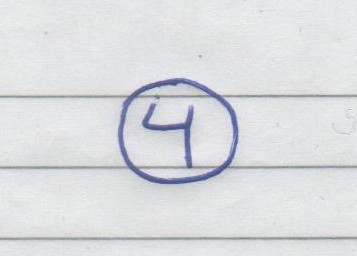
\includegraphics[width=0.7\textwidth]{./images/imagen1.jpg}
	\caption{Nodo raíz del árbol}
\end{figure} 
Continuando con la inserción de datos, en este caso el numero 7 se procede de la siguiente manera, primero se coloca un puntero sobre la raíz, si 
el valor de la raíz es menor que el valor a insertar se verifica que el nodo de la izquierda exista, si existe entonces se mueve el puntero a ese Nodo
y se repite el ciclo, si no existe se crea el nodo y se asigna al puntero izquierdo de el ultimo nodo la dirección de memoria del nodo creado, ahora
si el valor es mayor se realiza el mismo proceso pero esta vez en vez de moverse a la izquierda se mueve a la derecha. Ver Figura 2
\begin{figure}[H]
	\centering
	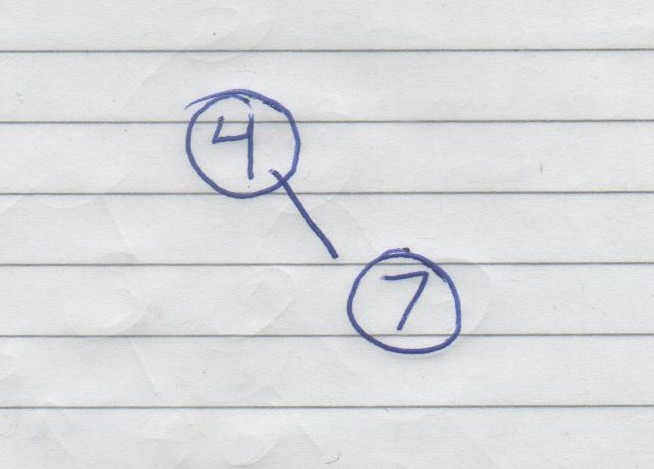
\includegraphics[width=0.7\textwidth]{./images/imagen2.jpg}
	\caption{Nodo raíz con una hoja a la derecha}
\end{figure} 
En las siguientes imágenes se puede ver el proceso de inserción, con una breve lista de los pasos seguidos
\\
2 menor que 4 entonces izquierda, se inserta en nodo vació
\begin{figure}[H]
	\centering
	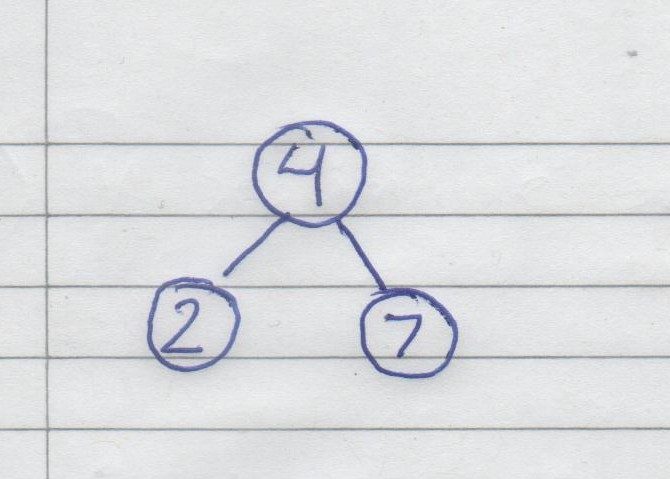
\includegraphics[width=0.7\textwidth]{./images/imagen3.jpg}
	\caption{Inserción del 2}
\end{figure} 
9 mayor que 4 entonces derecha, mayor que 7 entonces derecha, se inserta en nodo vacío
\begin{figure}[H]
	\centering
	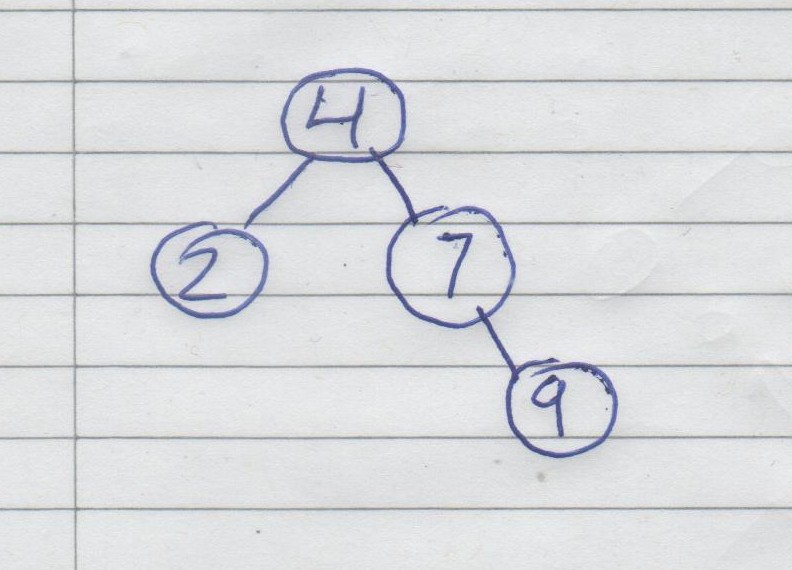
\includegraphics[width=0.7\textwidth]{./images/imagen4.jpg}
	\caption{Inserción del 9}
\end{figure}
5 mayor que 4 entonces derecha, menor que 7 entonces izquierda, se inserta en nodo vacío
\begin{figure}[H]
	\centering
	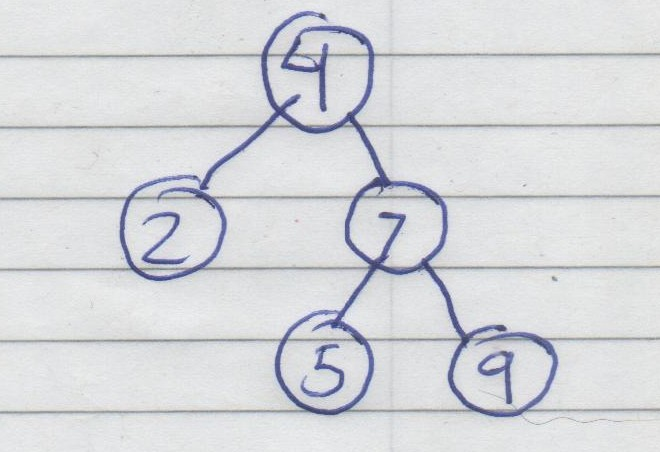
\includegraphics[width=0.7\textwidth]{./images/imagen5.jpg}
	\caption{Inserción del 5}
\end{figure} 
6 mayor que 4 entonces derecha, menor que 7 entonces izquierda,mayor que 5 entonces derecha, se inserta en nodo vacío
\begin{figure}[H]
	\centering
	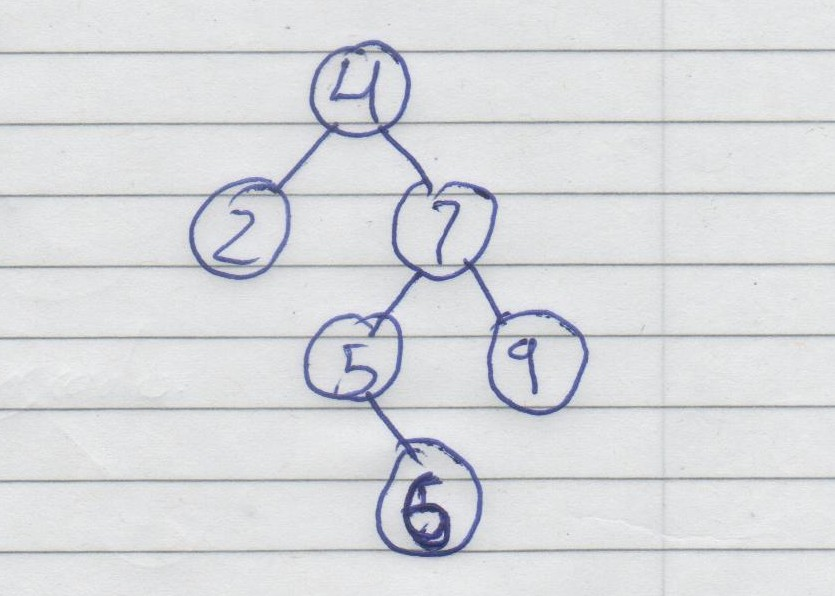
\includegraphics[width=0.7\textwidth]{./images/imagen6.jpg}
	\caption{Inserción del 6}
\end{figure} 
1 menor que 4 entonces izquierda, menor que 2 entonces izquierda, se inserta en nodo vacío
\begin{figure}[H]
	\centering
	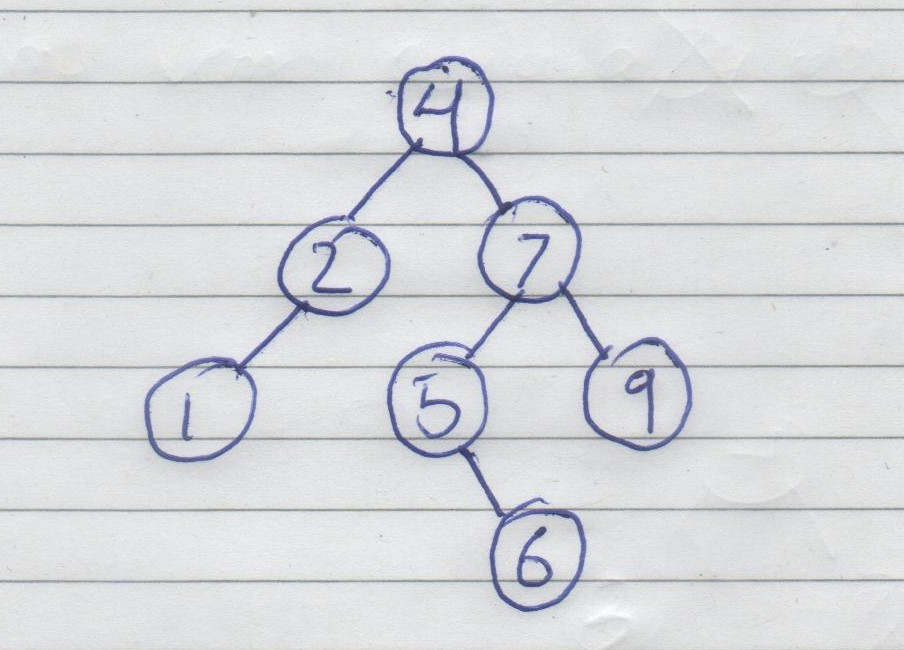
\includegraphics[width=0.7\textwidth]{./images/imagen7.jpg}
	\caption{Inserción del 1}
\end{figure} 
0 menor que 4 entonces izquierda, menor que 2 entonces izquierda,menor que 1 entonces izquierda, se inserta en nodo vacío

15 mayor que 4 entonces derecha, mayor que 7 entonces derecha,mayor que 9 entonces derecha, se inserta en nodo vacío
\begin{figure}[H]
	\centering
	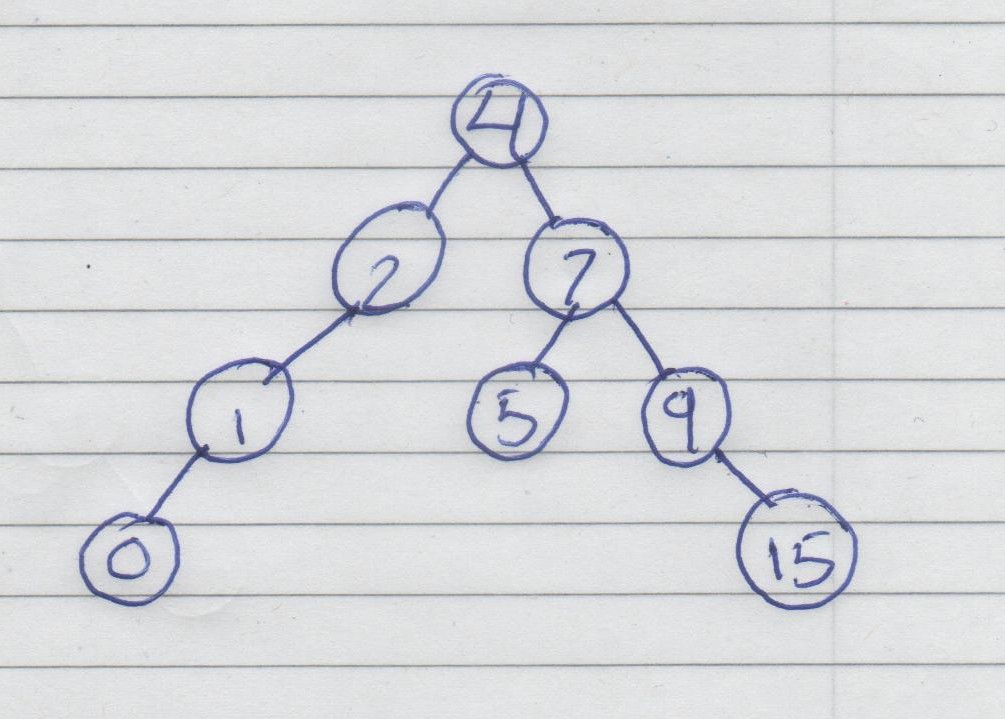
\includegraphics[width=0.7\textwidth]{./images/imagen8.jpg}
	\caption{Inserción del 0 y el 15}
\end{figure}
3 menor que 4 entonces izquierda, mayor que 2 entonces derecha, se inserta en nodo vacío
\begin{figure}[H]
	\centering
	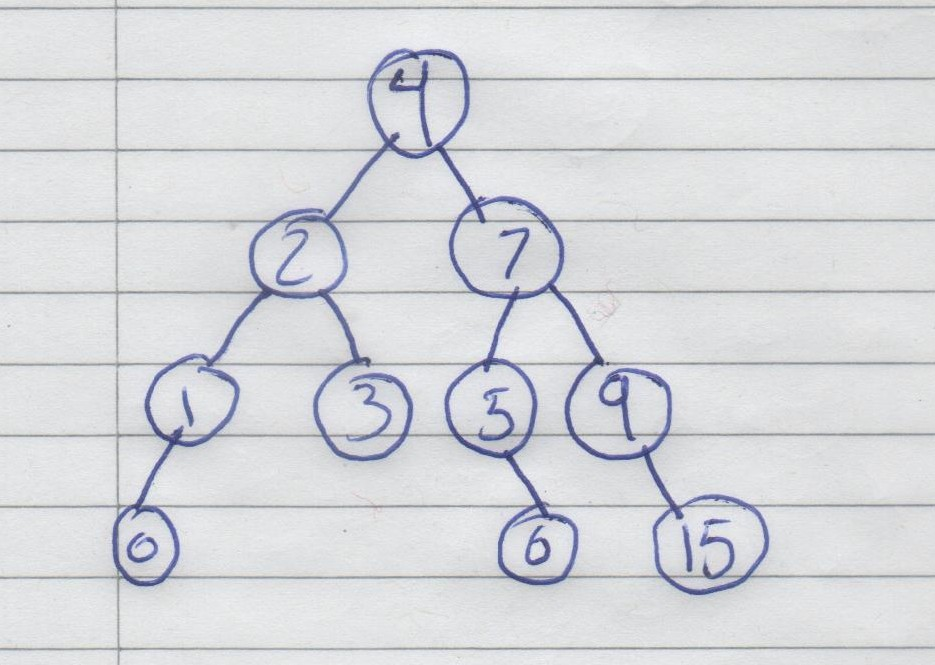
\includegraphics[width=0.7\textwidth]{./images/imagen9.jpg}
	\caption{Inserción del 3}
\end{figure} 
\subsubsection{Borrado}
Para borrar un nodo es necesario realizar dos búsquedas, la primera es buscar el nodo mayor a la izquierda del nodo a borrar, y la segunda es buscar el nodo
menor a la derecha del nodo a borrar, si ambas existen entonces se puede escoger entre cualquiera, si no entonces se escoge la verdadera y se sustituye 
por el valor correspondiente, si el mayor a la izquierda o el menor a la derecha tienen hijos, es necesario realizar el proceso recursivamente, entonces en el 
ejemplo podemos realizar el borrado del 2, primero nos posicionamos sobre el numero correspondiente, realizamos ambas búsquedas, en este caso ambas existen,
el mayor a la izquierda es el numero 1 y el menor a la derecha es el 3 como ambas existen entonces se puede usar cualquiera de las dos,
si usamos el 3 por ejemplo simplemente es asignar el valor 3 al nodo donde esta el 2 y borrar el nodo 3, así logramos el resultado de la Figura 10.
\begin{figure}[H]
	\centering
	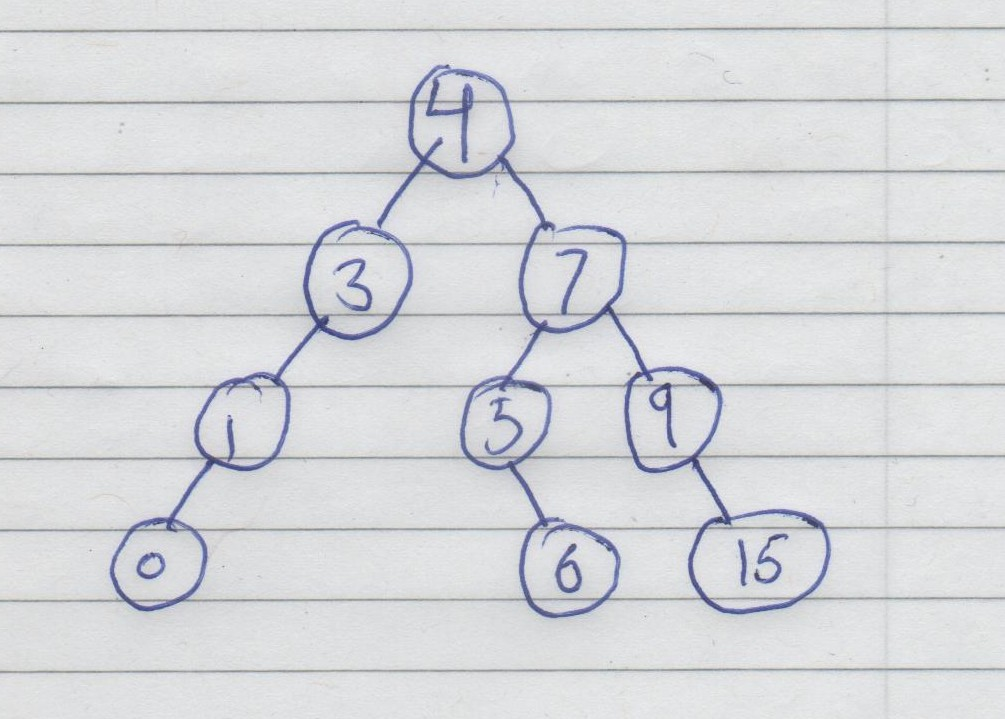
\includegraphics[width=0.7\textwidth]{./images/imagen10.jpg}
	\caption{Borrado del 2}
\end{figure} 
Para borrar el numero 6 realizamos el mismo procedimiento, buscamos el mayor a la izquierda y el menor a la derecha, como en este caso ninguno de los dos existe
quiere decir que el 6 es una hoja, como no tiene hijos simplemente se borra, sucede lo mismo con el 0 y el 15. Así borrando los 3 números el resultado escoge
el de la Figura 11
\begin{figure}[H]
	\centering
	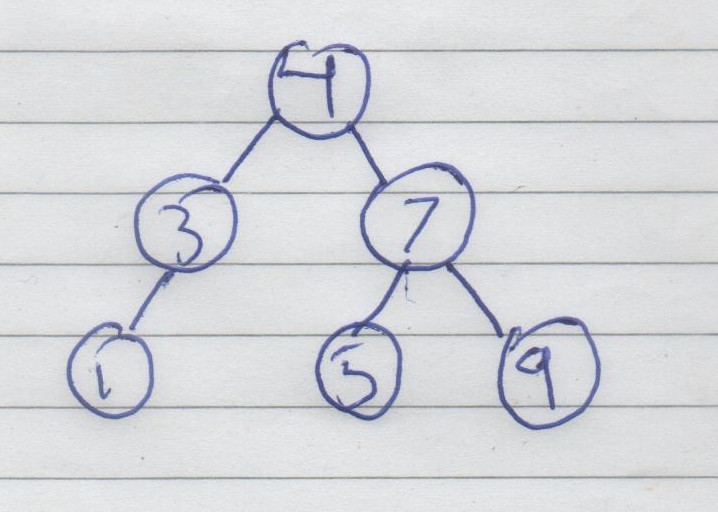
\includegraphics[width=0.7\textwidth]{./images/imagen11.jpg}
	\caption{Borrado del 6, del 0, del 15}
\end{figure} 
\subsubsection{Balanceo}
Para balancear lo mas fácil es crear un nuevo árbol a partir de el árbol desvalanceado, para esto primero se hace una lista con los números del árbol
como en la Figura 12
\begin{figure}[H]
	\centering
	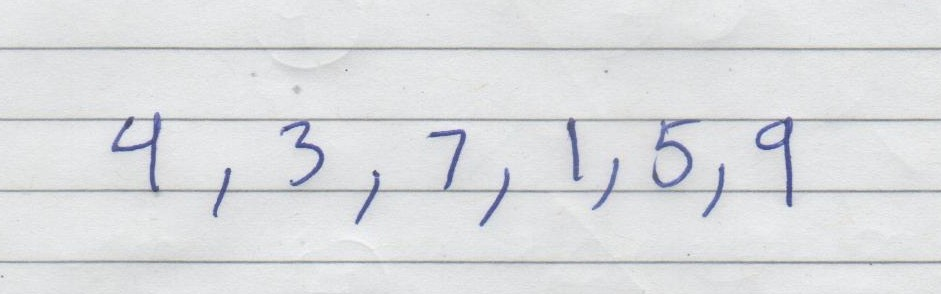
\includegraphics[width=0.7\textwidth]{./images/otraimagen1.jpg}
	\caption{Lista de números}
\end{figure}
Después se acomodan en orden de menor a mayor. Ver Figura 13
\begin{figure}[H]
	\centering
	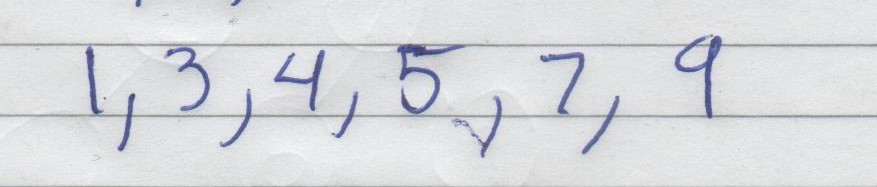
\includegraphics[width=0.7\textwidth]{./images/otraimagen2.jpg}
	\caption{Lista de números ordenados}
\end{figure}
Con la lista acomodada basta realizar el siguiente proceso, se busca el valor del medio en este caso puede ser 4 o 5, tomamos el 5 y lo insertamos como en la Figura
14, después recursivamente seguimos con el mismo proceso buscamos la mitad de la mitad en este caso el 3 (Figura 15), después la mitad derecha que seria el 7 (Figura 16)
y así sucesivamente hasta terminar con la lista
\begin{figure}[H]
	\centering
	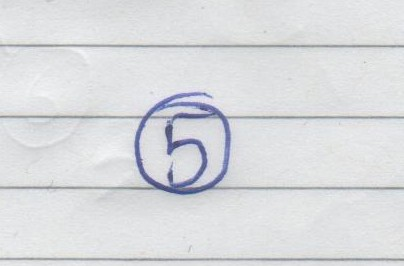
\includegraphics[width=0.7\textwidth]{./images/otraimagen3.jpg}
	\caption{Inserción del 5}
\end{figure}
\begin{figure}[H]
	\centering
	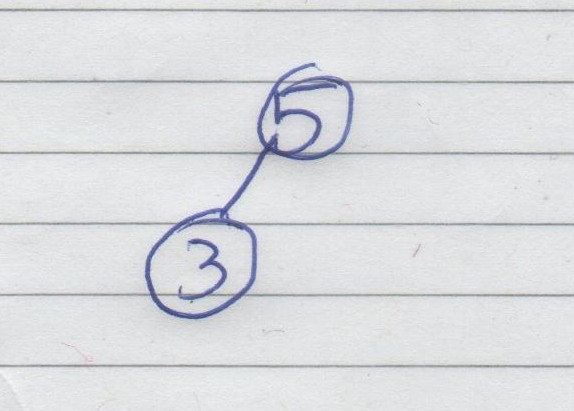
\includegraphics[width=0.7\textwidth]{./images/otraimagen4.jpg}
	\caption{Inserción del 3}
\end{figure}
\begin{figure}[H]
	\centering
	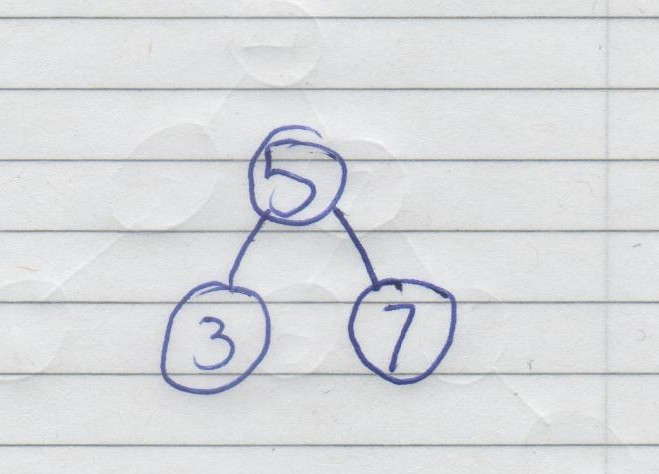
\includegraphics[width=0.7\textwidth]{./images/otraimagen5.jpg}
	\caption{Inserción del 7}
\end{figure}
\begin{figure}[H]
	\centering
	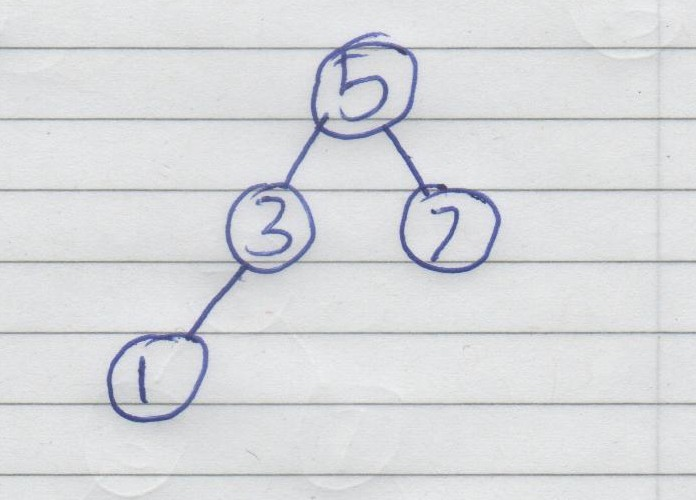
\includegraphics[width=0.7\textwidth]{./images/otraimagen6.jpg}
	\caption{Inserción del 1}
\end{figure}
\begin{figure}[H]
	\centering
	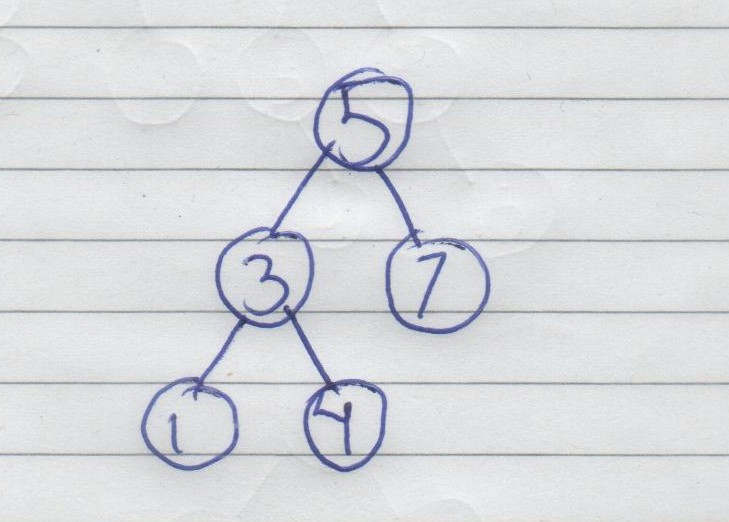
\includegraphics[width=0.7\textwidth]{./images/otraimagen7.jpg}
	\caption{Inserción del 4}
\end{figure}
\begin{figure}[H]
	\centering
	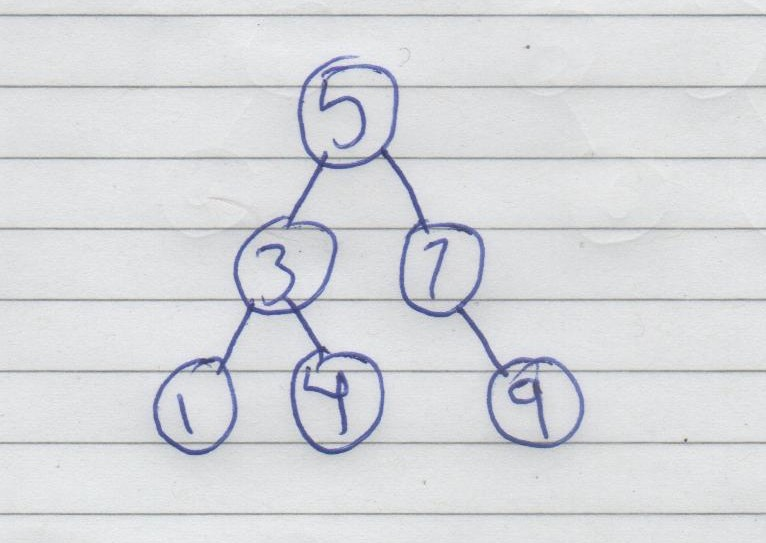
\includegraphics[width=0.7\textwidth]{./images/otraimagen8.jpg}
	\caption{Inserción del 9}
\end{figure}
Al finalizar el proceso el árbol queda balanceado.
\section{Conclusiones}
Después de desarrollar esta tarea se logro concluir
\begin{itemize}
	\item El manejo de pilas y colas es muy importante para manejar el orden de ejecución de procesos
	\item Son modelos relativamente sencillos y debido a su simpleza son muy cómodos de trabajar
	\item Un árbol binario puede realizar búsqueda de información en un tiempo muy reducido
\end{itemize}
